% Template for ICASSP-2016 paper; to be used with:
%          spconf.sty  - ICASSP/ICIP LaTeX style file, and
%          IEEEbib.bst - IEEE bibliography style file.
% --------------------------------------------------------------------------
\documentclass{article}

\usepackage{spconf,amsmath,graphicx,siunitx,booktabs}
\usepackage{varioref}

% Example definitions.
% --------------------
\def\x{{\mathbf x}}
\def\L{{\cal L}}

% Title.
% ------
\title{Speech Language Recognition Combining Phoneme Detection Statistical Analysis and Neural Networks}
%
% Single address.
% ---------------
\name{Quentin Deleuil, Gianmarco Garrisi, Qianyun Hu, Patrik Scheible \thanks{Thanks to XYZ agency for funding.}}
\address{quentin.deleuil@gmail.com, s212260@studenti.polito.it, patrikscheible@posteo.net, }
%
% For example:
% ------------
%\address{School\\
%	Department\\
%	Address}
%
% Two addresses (uncomment and modify for two-address case).
% ----------------------------------------------------------
%\twoauthors
%  {A. Author-one, B. Author-two\sthanks{Thanks to XYZ agency for funding.}}
%	{School A-B\\
%	Department A-B\\
%	Address A-B}
%  {C. Author-three, D. Author-four\sthanks{The fourth author performed the work
%	while at ...}}
%	{School C-D\\
%	Department C-D\\
%	Address C-D}
%
\begin{document}
%\ninept
%
\maketitle
%
\begin{abstract}

\end{abstract}
In this project, we explore two techniques to identify spoken language. For one system, we extract the phonemes from audio files and use Phonemes Statistical Analysis(PSA) approach to classify languages. For the other, audios files are transformed into Mel-frequency Cepstral Coefficients (MFCC) images. And we construct a Deep Neural Network (DNN) to identify languages. We used Arabic, Dutch, Korean, Polish and Romanian as languages to recognise. Both systems reach a higher accuracy than 93\%. 

\begin{keywords}
Language Identification, Phonemes, CMUSphinx, Deep Neural network
\end{keywords}
%
\section{Introduction}
\label{sec:intro}
Spoken language identification is to classify the spoken language from a given audio sample, which is typically the first step for language processing tasks. Without spoken language identification, speech utterances cannot be analyzed correctly and the grammar rules cannot be applied. As with speech recognition, humans can perform the most accurate language identification.\cite{shi2006importance} Within a few seconds of hearing, people are able to identify if they have prior knowledge of this language. In the other case, people can just make subjective judgements to the similarity of the language they know.

There are several critical applications for spoken language identification, such as international emergency call for urgent occasions and language predefined for intelligent assistants like Siri. 
Thus, a spoken language identification system should be developed for such cases.

In our project, we explore two different approaches, Phoneme Statistical Analysis (PSA) and Deep Neural Network (DNN), to identifying the language of speech. In the PSA approach, we extract the phonemes and build a statistical analysis model for each language. While in DNN approach, we transform information from the audio signal to Mel-frequency Cepstral Coefficients (MFCC) and use Convolutional Neural Network (CNN) combined with Recurrent Neural Network (RNN) to train the system.

The report is structured in the following way: In Section~\ref{sec:psa} we introduce the system of PSA. The approach with DNN will be shown in Section~\ref{sec:dnn}. In Section~\ref{sec:comparision} we compare the systems and suggest a method of combining them and finally show our conclusions in Section~\ref{sec:conclusion}. 

\section{Dataset}
\label{sec:dataset}
The data comes from the \textit{TopCoder} competition on language identification. It includes 66,176 labelled samples of 10 seconds of spoken language in 176 languages in \textit{mp3} format, sampled at 16\,kHz. From this data set we selected the five languages Arabic,  Dutch,  Korean,  Polish  and  Romanian with 376 labelled samples each. Then we split it into training and test set with a 70\,\% -- 30\,\% ratio. All samples were converted into raw (\textit{.wav}) format for easier processing in Python.

\section{Phoneme Statistical Analysis}
\label{sec:psa}
\subsection{Techniques}
The first step in this approach is to convert all audio files in the training set into their corresponding phonemes using the framework CMU Sphinx \cite{lamere2003cmu} and Python. Since the project scope does not allow to create a neutral language model for CMU Sphinx the standard American English model is used. Thus rather low performance of the actual phoneme recognition can be expected \cite{kepuska2017comparing}. However our assumption is that a certain language produces a specific pattern of phonemes even though these phonemes are not the real phonemes of the utterance. Thus the real phonemes are not of interest, just the pattern of (wrong) phonemes that a certain language produces in this phoneme recogniser. The output of this step is one text file per language containing the phonemes of one sample in each line.

In the second step, n-grams of the phonemes of each language are computed. \cite{matejka2005phonotactic} used 3-grams to model a language, however this requires more training data than for this project is available. Therefore histograms (1-grams) and 2-grams are considered.

After training the model, the phonemes of a data sample have to be compared to the statistical models of each language. This can be done by computing the likelihood of the sample per language \cite{matejka2005phonotactic} as in equation (\ref{equ:likelihood}) with $\theta$ being the language, $x$ being the sample, $x_i$ being the i\textit{th} phoneme of sample $x$ and $p_{\theta}(\cdot)$ being the histogram of the language $\theta$.

\begin{equation}
\label{equ:likelihood}
    \mathcal{L}(\theta | x) = \prod p_{\theta} (x_i)
\end{equation}

A second method for comparison with the likelihood is to calculate the Kullback-Leibler Distance between the models histogram and the sample's histogram as shown in Equation~(\ref{equ:kullback-leibler}) where $P$ is the model's histogram and $Q$ is the sample's histogram.

\begin{equation}
\label{equ:kullback-leibler}
    D(P || Q) = - \sum_{i} P(i) log\left(\frac{Q(i)}{P(i)}\right)
\end{equation}

Finally the language with the highest likelihood or with the lowest distance is selected as the estimation.

\subsection{Experiments}

After training 1-gram models, the distance between the language models can give some initial insight if they represent good models for discrimination. Figure~\ref{fig:distance_between_languages} is a plot that shows the Kullback-Leibler distance (Equation~(\ref{equ:kullback-leibler})) between each of the models. For instance it reveals that Arabic and Polish are more different than Korean and Romanian.

\begin{figure}[h]
    \centering
    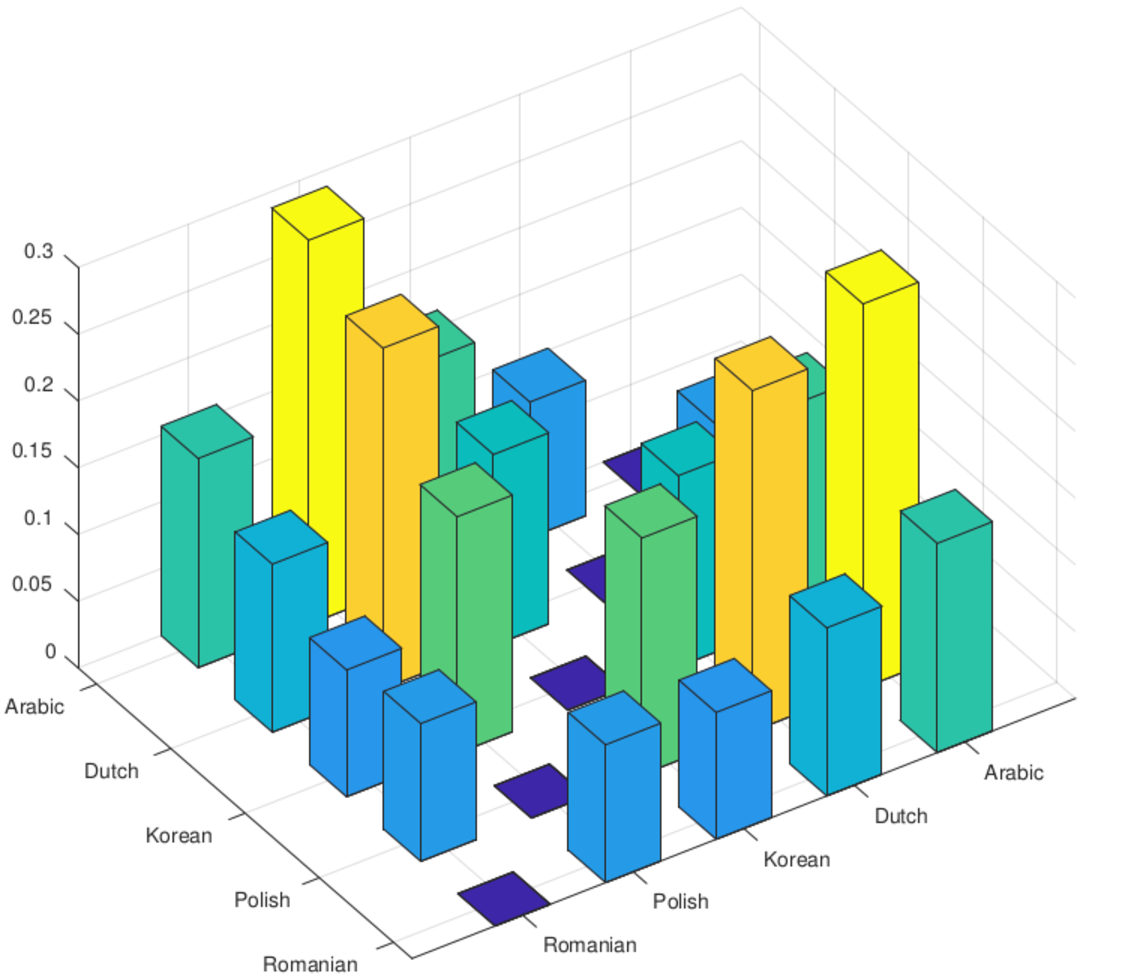
\includegraphics[width=0.48\textwidth]{img/kullback-leibler_5languages.pdf}
    \caption{Kullback-Leibler Distance between the trained models.}
    \label{fig:distance_between_languages}
\end{figure}

In the next step the two distance functions are evaluated on the test set. Here both, equation~(\ref{equ:likelihood})~and~(\ref{equ:kullback-leibler}) yield exactly the same confusion matrix, given in Table~\ref{tab:confusion_matrix_psa}. The accuracy is 93.27\,\%.

\begin{table}[h]
\begin{center}
\begin{tabular}{ l | r r r r r }
          & Arabic & Dutch & Korean & Polish & Rom.\\
\hline
 Arabic   & 112    & 0     & 0      & 0      & 1\\
 Dutch    & 3      & 106   & 1      & 0      & 3\\
 Korean   & 2      & 0     & 99     & 5      & 7\\
 Polish   & 0      & 0     & 1      & 105    & 7\\
 Romanian & 0      & 4     & 3      & 1     & 105\\
\end{tabular}
\end{center}
\caption{Confusion Matrix with PSA using Kullback-Leibler distance and Likelihood (both yield the same matrix). }
\label{tab:confusion_matrix_psa}
\end{table}

Conducting the same experiments with 2-gram models yields an accuracy of only 55.22\,\%. For example the Polish language model contains 1763 2-grams. However it contains 274 2-grams that are not present and 231 2-grams that only appeared once in the training set. This is an indication that not enough training data was used to get a true realisation of the underlying statistic.

\begin{table}[h]
\begin{center}
\begin{tabular}{ l | r r r r r }
          & Arabic & Dutch & Korean & Polish & Rom.\\
\hline
 Arabic   & 108    & 1     & 0      & 1      & 2\\
 Dutch    & 4      & 103   & 1      & 3      & 1\\
 Korean   & 0      & 0     & 110    & 2      & 0\\
 Polish   & 5      & 4     & 1      & 98    & 4\\
 Romanian & 3      & 0     & 0      & 0     & 109\\
\end{tabular}
\end{center}
\caption{Confusion Matrix with CRNN}
\label{tab:confusion_matrix_crnn}
\end{table}

\section{Deep Neural Networks}
\label{sec:dnn}
In this section we identify the spoken language with two architectures of Deep Neural Networks. At first stage we extract the audio features as \emph{Mel-frequency cepstral coefficients} (MFCC) representation using the librosa library. The librosa library was also used to perform data augmentation.
 
Then the MFCCs are used as input for the CRNN created with the Keras framework.

\subsection{Techniques}
\label{subsec:dnn-tech}
We represented the audio samples using MFCCs with 40 bands. The resulting matrices have a shape of $(40, 443)$.

To limit the \emph{overfitting} problem, we also implemented \emph{data augmentation} producing, for each input file in the training set, three versions differing in the speed of the voice: the original file, a version with a slight slowdown and another one slightly faster. To easily feed the network with these data, we cropped the longer files (the slower ones) and zero padded the faster, producing at the end matrices with a fixed shape.
Eventually, the three versions have a relative speeds of $0.9$, $1$ and $1.1$ times the original version.

There was also the possibility that the resulting MFCCs had a resolution too high in time, that would have made the training of the neural network too slow, so we thought to the possibility of reducing the dimensionality in time domain. In fact, that was not the case, with a training time taking around \SI{35}{\milli\second} per step. 

For what concerns the neural networks, we tried two types of them: a more classical \emph{Convolutional Neural Network} (CNN), and a \emph{Convolutional Recurrent Neural Network} (CRNN), that is a CNN with one or more \emph{Long Short-term Memory} layers after the convolutional part and before the fully connected layers. Long short-term memory (LSTM) units are units of a recurrent neural network (RNN) . A LSTM unit composed a cell, an input gate, an output gate and forget gate. It is well-suited to classifying based on time series data.

In both cases we used three convolutional layers followed each by a maxpooling layer, two dense layers and a dropout layer to reduce overfitting. For the CRNN we added an LSTM layer after the convolutional layers and before the fully connected ones. 

\subsection{Experiments}
\label{subsec:dnn-experiments}

\subsubsection{Convolutional Neural Network}
As a first attempt, we tried to implement a standard CNN with 3 blocks with configuration of neurons 32-32-64, composed each by a Convolutional layer with filters of size $3\times 3$ and a maxpooling layer with stride 2, at the end two fully connected layers with size 64 and 5 for the output and a \emph{dropout} layer between them.
\begin{figure}[h]
    \centering
    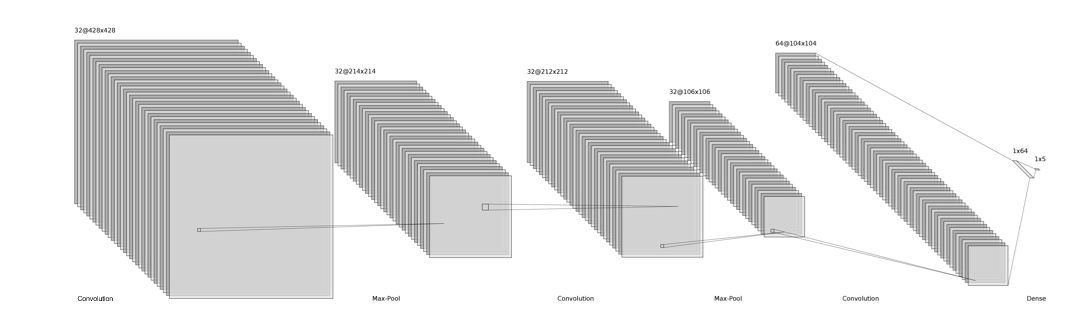
\includegraphics[width=0.5\textwidth]{img/cnn_figure.PNG}
    \caption{Convolutional Neural Network model}
    \label{fig:CNN model}
\end{figure}

We chose the \emph{ReLU} as the activation function and \emph{RMSprop} as optimizer. The loss function is the \emph{categorical cross-entropy}. The dataset has been split between a training set and a test set respectively equal to the \SI{70}{\percent} and \SI{30}{\percent}.

After 20 epochs of training over the non-augmented dataset, this model reached an accuracy of \SI{89.7}{\percent} on the test set.
Dispite the dropout layer, this result is affected by overfitting. At the last epoch in fact, the accuracy on the training set gets over \SI{98}{\percent}.

To improve it, we implemented data augmentation, as explained in Section \ref{subsec:dnn-tech}. We also split the dataset into three sets: one for training, one for validation and one for the testing phase with a proporttion of \SI{56}{\percent}, \SI{14}{\percent}  and \SI{30}{\percent}. We used a technique to save the weights of the best network according to the value of the loss function on the validation set. We later use the best model for the evaluation phase.

We were able to train the network for 30 epochs without overfitting reaching an accuracy of over \SI{95}{\percent} on the validation set and  on the test set.

From the confusion matrix results that our network is very good at detecting Korean and Romanian.

\subsubsection{Convolutional Recurrent Neural Network}
To improve the network, based on the CNN structure, we implement a Long Short-Term Memory (LSTM) layer with 64 neurons. The accuracy improve to \SI{93.75}{\percent}

To improve the network, based on the CNN structure, we implement a Long Short-Term Memory (LSTM) layer with 64 neurons. 
The accuracy improve to \SI{93.75}{\percent}, training the network on the augmented dataset.
Because of the network architecture and the software implementation we have to discard a small part of the sets. It is a number of samples less than the number of elements in a minibatch and is distributed among all the languages.

In our case this amounts to less then 64 samples, which should not impact the overall performance of the network.

All the obtained results are reported in \tablename~\ref{tab:dnn-acc-comp}. The confusion matrix for the CRNN is in \tablename~\ref{tab:confusion_matrix_crnn}.

\begin{table}
  \centering
  \begin{tabular}{lcr}
    \toprule
    Architecture & Data augmentation & Accuracy (\si{\percent}) \\
    \midrule
    Convolutional & No & 89.7 \\
    Convolutional & Yes & 95.17 \\
    Conv. Recurrent & Yes & 93.75 \\
    \bottomrule
  \end{tabular}
  \caption{Comparison of accuracy between different networks}\label{tab:dnn-acc-comp}
\end{table}

\section{Comparison of the two Systems}
\label{sec:comparision}

Both systems show a similar performance on the test set, no systems proofs to be superior over the other. However, comparing the diagonals of the confusion matrices for both systems in Table~\ref{tab:confusion_matrix_psa} and Table~\ref{tab:confusion_matrix_crnn} we see that each system has languages it works better with. For instance Korean has 110 true positives in the CRNN and only 99 true positives in the PSA.

Considering that when we input a sample into each system, the result are 5 likelihoods. To further improve the performance a weighted average between these likelihoods can be applied. Therefore, first the likelihoods have to be normalised and then the system that performs better on the test data has to get the higher weight. This yields five final likelihoods from which the highest is the estimated language.

To test this approach, it is necessary to use a new test set, since the weights are based on the original test set. This is left as future work, since the data basis available for this project is not large enough.

\section{Conclusions}
\label{sec:conclusion}

In this project we propose two spoken language identification systems for five languages from different language families. In the PSA system, we extract phonemes and build a statistical model for each language. While in the DNN system, we first convert the audio domain into image domain with MFCC features. Then we propose a CNN structure with data augmentation and a CRNN structure with a LSTM layer based on CNN. 
We could show that performing PSA shows almost the same performance as a DNN. (CANG)

Also a data set is not large enough to apply 2-gram models, therefore with more data a even higher performance in the PSA approach can be expected. Using a phoneme recognizer that is known to only exhibit low performance (using wrong language models) has proved to be still a useful tool to language identification.

For the DNN system, a simple structure predict a high accuracy due to the preprocessing of MFCC. The accuracy improved after data augmentation of training set. Other network structures can be tried to further improve the performance.

Finally, we can try to combine both systems to get the best of both. One way this can be done is looking at the results and assign weights to the predictions of both systems.
%\section{REFERENCES}
%\label{sec:refs}


% References should be produced using the bibtex program from suitable
% BiBTeX files (here: strings, refs, manuals). The IEEEbib.bst bibliography
% style file from IEEE produces unsorted bibliography list.
% -------------------------------------------------------------------------
\bibliographystyle{IEEEbib}
\bibliography{refs}

\end{document}
